\documentclass[border=10pt]{standalone}
% Shared style for the EMONI diagrams. Build: tectonic <file>.tex, then pdftocairo -svg.
\usepackage{fontspec}
\setmainfont{FiraSans}[Extension=.otf,UprightFont=*-Regular,BoldFont=*-SemiBold,ItalicFont=*-Italic,BoldItalicFont=*-SemiBoldItalic]
\setmonofont{FiraMono}[Extension=.otf,UprightFont=*-Regular,BoldFont=*-Medium,Scale=0.9]
\usepackage{tikz}
\usetikzlibrary{arrows.meta,positioning,shapes.geometric,shapes.misc,calc,fit,backgrounds}
\definecolor{eg}{HTML}{11903B}   % EMONI green
\definecolor{egl}{HTML}{E8F7EE}
\definecolor{eb}{HTML}{2A78D6}   % blue
\definecolor{ebl}{HTML}{EAF2FC}
\definecolor{eo}{HTML}{D9631E}   % orange
\definecolor{eol}{HTML}{FDF0E7}
\definecolor{ep}{HTML}{7C4DCC}   % purple
\definecolor{epl}{HTML}{F2ECFB}
\definecolor{er}{HTML}{C5221F}   % red
\definecolor{erl}{HTML}{FCEAEA}
\definecolor{ink}{HTML}{1F2328}
\definecolor{mute}{HTML}{59636E}
\definecolor{line}{HTML}{D0D7DE}
\tikzset{
  every node/.style={text=ink,font=\small},
  >={Stealth[length=2.4mm]},
  % sequence diagrams
  life/.style={draw=line,dashed,thick},
  head/.style={draw=#1,fill=#1!8,rounded corners=3pt,minimum width=27mm,minimum height=11mm,align=center,font=\small\bfseries,thick},
  act/.style={draw=#1,fill=#1!18,minimum width=2.2mm},
  msg/.style={->,thick,draw=ink},
  ret/.style={->,dashed,draw=mute},
  mlabel/.style={font=\footnotesize,fill=white,inner sep=1.5pt,align=center},
  note/.style={draw=#1,fill=#1!8,rounded corners=2pt,font=\footnotesize,align=left,inner sep=4pt},
  frag/.style={draw=mute,rounded corners=2pt},
  fraglabel/.style={draw=mute,fill=white,font=\footnotesize\bfseries,inner sep=2.5pt,anchor=north west},
  % activity diagrams
  start/.style={circle,fill=ink,minimum size=4mm,inner sep=0},
  stop/.style={circle,draw=ink,thick,minimum size=5mm,inner sep=0,path picture={\fill[ink] (path picture bounding box.center) circle (1.4mm);}},
  step/.style={draw=#1,fill=#1!8,rounded corners=5pt,thick,minimum height=9mm,minimum width=40mm,align=center,font=\small},
  step/.default=eg,
  dec/.style={diamond,aspect=2.2,draw=ink,fill=white,thick,inner sep=1.5pt,align=center,font=\footnotesize},
  flow/.style={->,thick,draw=ink},
  guard/.style={font=\footnotesize\itshape,text=mute,fill=white,inner sep=1.5pt},
  lane/.style={draw=line,fill=#1,rounded corners=4pt},
  lanetitle/.style={font=\small\bfseries,text=mute},
}

% Sequence: a delta firmware update over LoRaWAN class A (public TRM, section 5).
\begin{document}
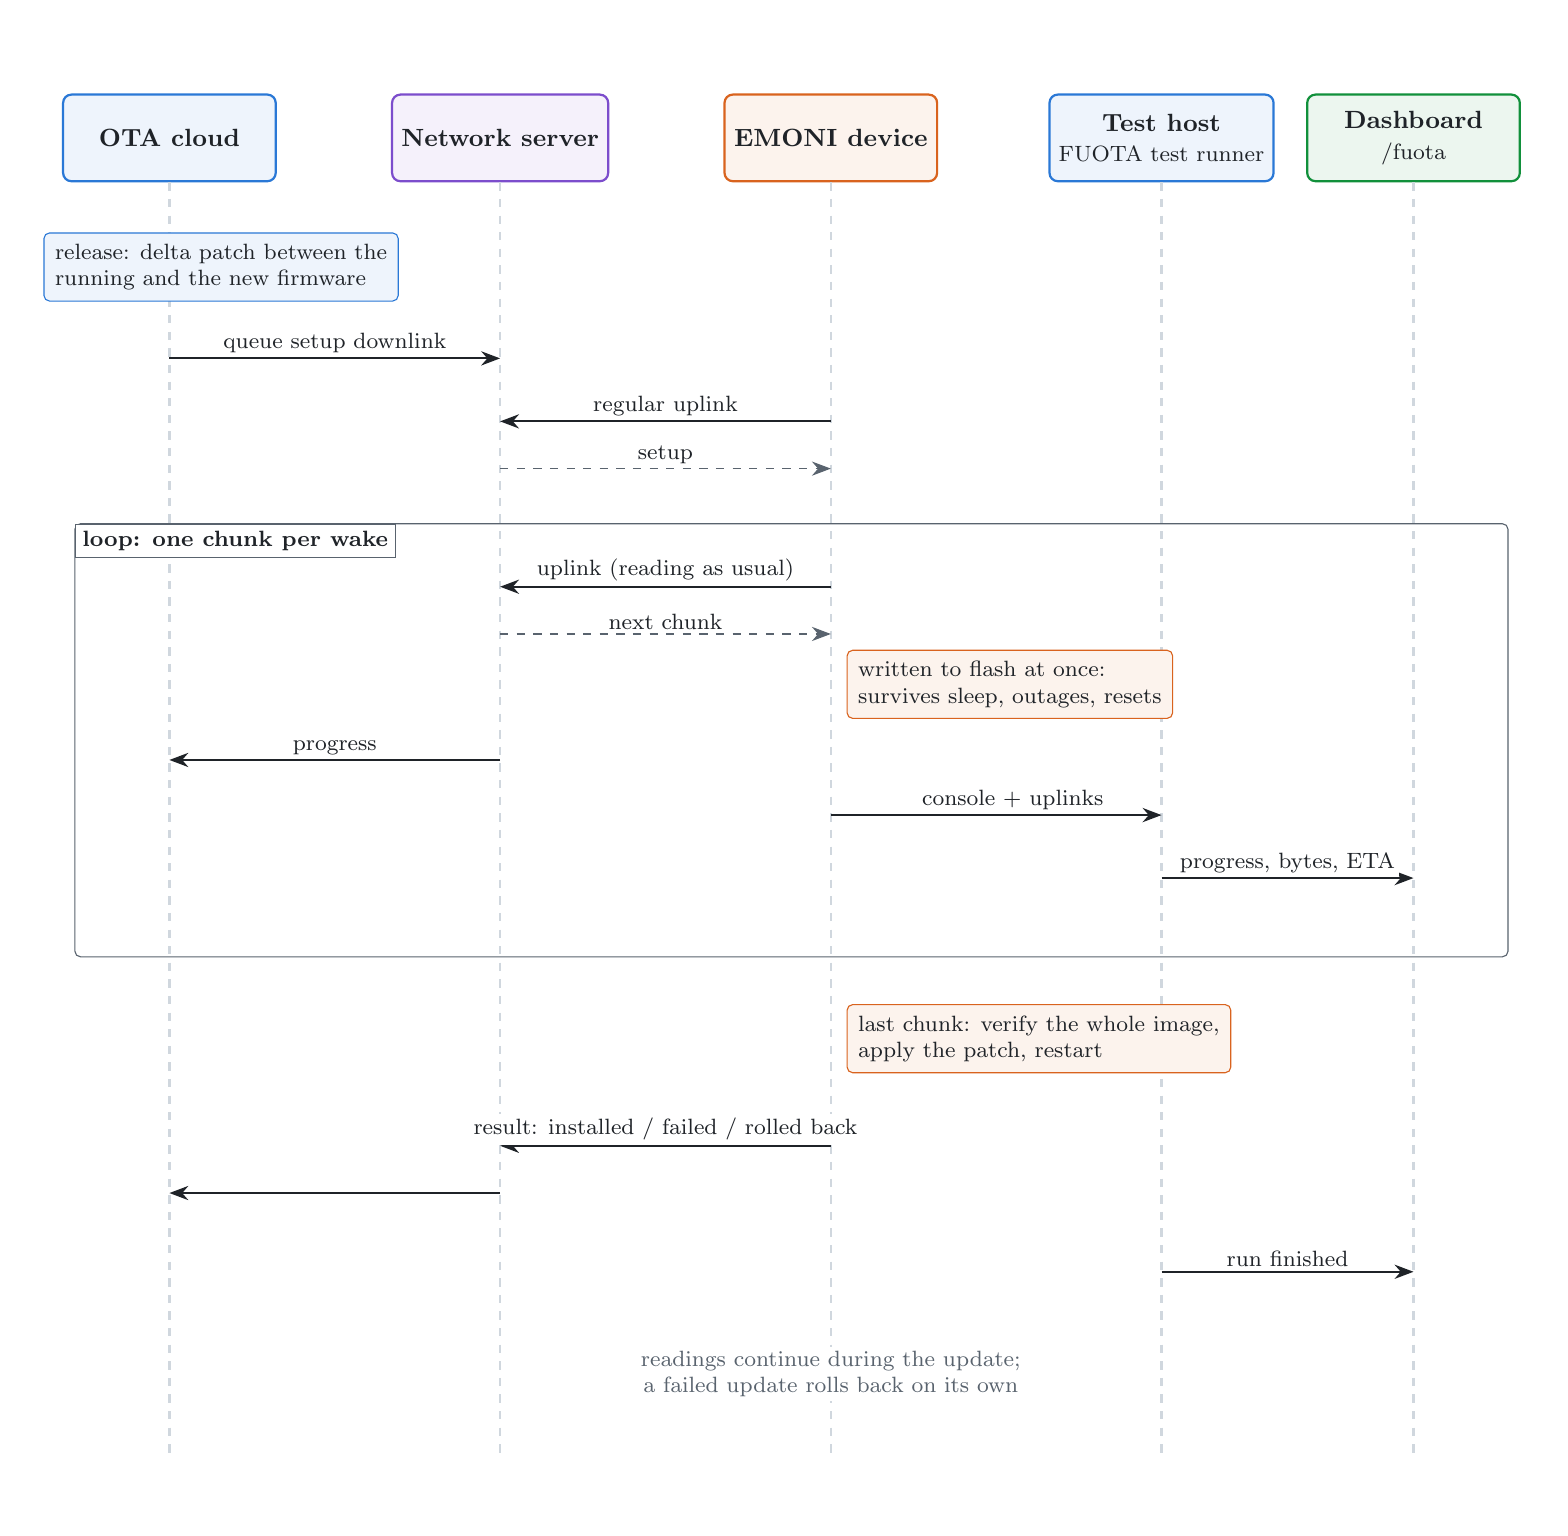
\begin{tikzpicture}[x=1cm,y=1cm]
\fill[white] (-1.8,1.4) rectangle (17.4,-17.4);
\def\B{-16.8}
\foreach \x/\n/\c/\t in {0/ota/eb/OTA cloud,
                         4.2/ns/ep/Network server,
                         8.4/dev/eo/EMONI device,
                         12.6/hil/eb/Test host\\{\footnotesize\mdseries FUOTA test runner},
                         15.8/dash/eg/Dashboard\\{\footnotesize\mdseries /fuota}}{
  \node[head=\c] (\n) at (\x,0) {\t};
  \draw[life] (\n.south) -- (\x,\B);
}
\node[note=eb,anchor=north west] at (-1.6,-1.2) {release: delta patch between the\\running and the new firmware};
\draw[msg] (0,-2.8) -- node[mlabel,above]{queue setup downlink} (4.2,-2.8);
\draw[msg] (8.4,-3.6) -- node[mlabel,above]{regular uplink} (4.2,-3.6);
\draw[ret] (4.2,-4.2) -- node[mlabel,above]{setup} (8.4,-4.2);
\draw[frag] (-1.2,-4.9) rectangle (17.0,-10.4);
\node[fraglabel] at (-1.2,-4.9) {loop: one chunk per wake};
\draw[msg] (8.4,-5.7) -- node[mlabel,above]{uplink (reading as usual)} (4.2,-5.7);
\draw[ret] (4.2,-6.3) -- node[mlabel,above]{next chunk} (8.4,-6.3);
\node[note=eo,anchor=north west] at (8.6,-6.5) {written to flash at once:\\survives sleep, outages, resets};
\draw[msg] (4.2,-7.9) -- node[mlabel,above]{progress} (0,-7.9);
\draw[msg] (8.4,-8.6) -- node[mlabel,above,pos=0.55]{console + uplinks} (12.6,-8.6);
\draw[msg] (12.6,-9.4) -- node[mlabel,above]{progress, bytes, ETA} (15.8,-9.4);
\node[note=eo,anchor=north west] at (8.6,-11.0) {last chunk: verify the whole image,\\apply the patch, restart};
\draw[msg] (8.4,-12.8) -- node[mlabel,above]{result: installed / failed / rolled back} (4.2,-12.8);
\draw[msg] (4.2,-13.4) -- (0,-13.4);
\draw[msg] (12.6,-14.4) -- node[mlabel,above]{run finished} (15.8,-14.4);
\node[mlabel,text=mute,align=center] at (8.4,-15.7) {readings continue during the update;\\a failed update rolls back on its own};
\end{tikzpicture}
\end{document}
